\section{New formalism}

The new formalism must allow simple interactions between user readable data and ifficient construction of the RBA problem. The data is going to be written is XML format, inspired by SBML standards.

\subsection{Final differences between RBAv01 and new formalism}

\begin{table}[!h]
  \centering
  \begin{tabular}{|l|c|c|c|c|}
    \hline
           & RBAv01 & RBAv01 & RBAnew & RBAnew \\
           & mat12  & mat15  & mat12  & mat15 \\
    \hline
    Input files & \multicolumn{2}{c|}{Custom files} & \multicolumn{2}{c|}{XML files} \\
    & \multicolumn{2}{c|}{+ partially hard coded} & \multicolumn{2}{c|}{(nothing hard coded)} \\
    \hline
    Code length & \multicolumn{2}{c|}{$\simeq 3500$} & \multicolumn{2}{c|}{$\simeq 1500$} \\
    (commented) & \multicolumn{2}{c|}{($\simeq 1000$)} & \multicolumn{2}{c|}{($\simeq 500$)} \\
    \hline
    Parsing & 15s & 8s & 12s & 12s \\
    \hline
    Solving (23 rounds) & 15s & 5s & 1.5-2s & 1.5-2s \\
    \hline
    1 matrix update & 580ms & 100ms & 3-10ms & 3-10ms \\
    \hline
    1 CPLEX round & 50ms & 58ms & 50ms & 58ms \\
    \hline
  \end{tabular}
  \caption{Comparison between original algorithm (RBAv01) and new formalism (RBAnew). Because performance for the old algorithm depended on matlab version, we included performance for matlab R2012a (mat12) and R2015b (mat15).}
  \label{tab:new_old_comparison}
\end{table}

\reftabt{tab:new_old_comparison} shows the main differences between RBAv01 and the new algorithm. The new algorithm uses generic XML files and is thus easier to modify for the end user. Parsing files is less efficient than the original algoirthm but this is not very important as it is only done once. More important is the solving time, which is significantly lower than the original algorithm.

The new algorithm could be improved further by handling block-allocation more efficiently for sparse matrices, but current performance seems pretty good.

\subsection{Input data}

\paragraph{Metabolism file}
\begin{figure}[ht]
  \centering
  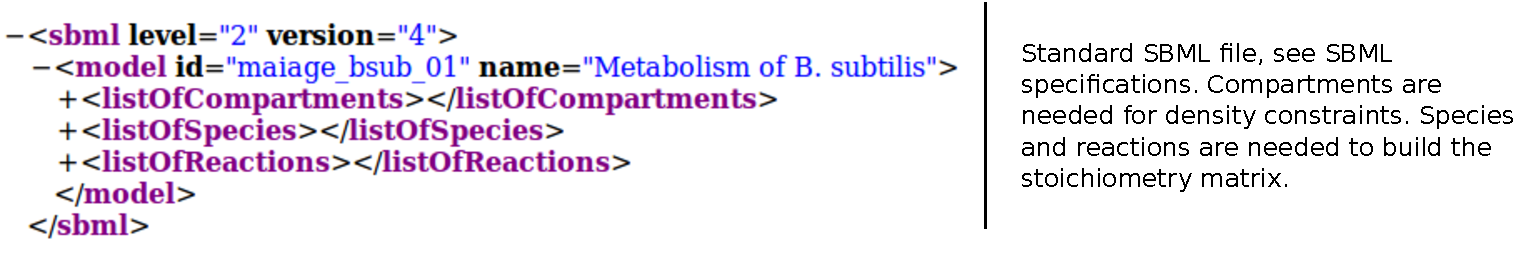
\includegraphics[width=\linewidth]{metabolism}
  \caption{Metabolism file is a standard SBML file.}
  \label{fig:metabolism}
\end{figure}
The metabolism file is a standard SBML file~\reffigp{fig:metabolism}. It contains information about cell compartments, metabolite species and metabolism reactions. Concentration of external metabolites are defined in the species section.

\paragraph{Parameter file}
\begin{figure}[ht]
  \centering
  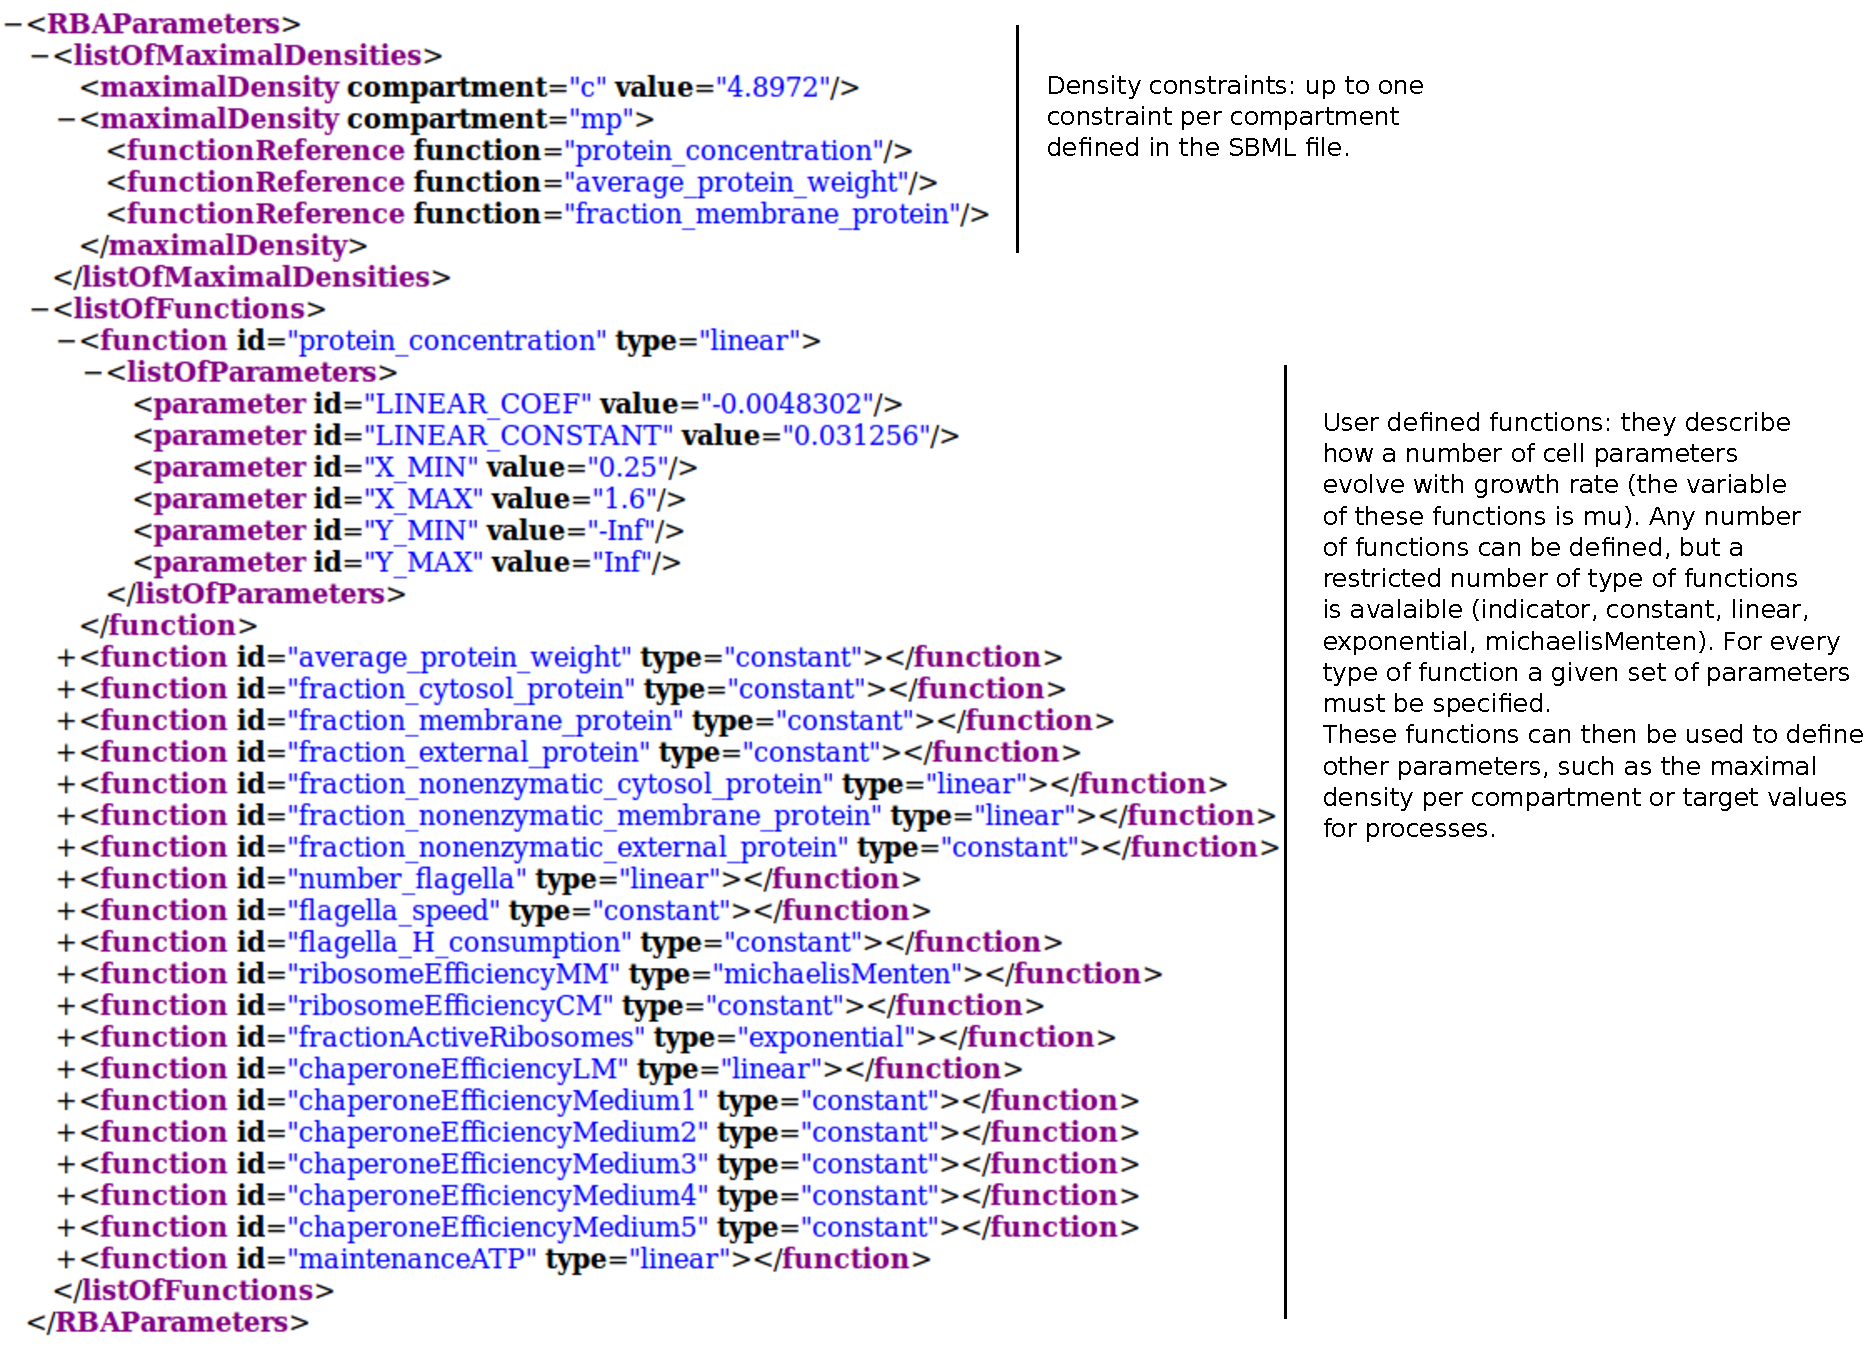
\includegraphics[width=\linewidth]{parameters}
  \caption{Structure of the parameter file used by RBA.}
  \label{fig:parameters}
\end{figure}
The parameter file is an XML file composed of two subsections~\reffigp{fig:parameters}. \texttt{listOfMaximalDensities} contains density constraints. \texttt{listOfFunctions} contains user-defined functions that can be used to set $\mu$-dependent maximal densities or $\mu$-dependent process targets (see below).

\paragraph{Macromolecule files}
\begin{figure}[ht]
  \centering
  \includegraphics[width=\linewidth]{proteins}
  \includegraphics[width=\linewidth]{rnadna}
  \caption{Structure of protein, RNA and DNA file.}
  \label{fig:proteins}
\end{figure}
Currently, RBA defines three sets of macromolecules: proteins, RNAs and DNA. One XML file is created for each set~\reffigp{fig:proteins}. All macromolecules have a \texttt{listOfComponents} describing the building blocks used to produce them (\textit{e.g.} amino acids, vitamins and ions for proteins). Then a \texttt{listOfSpecies} contains all molecules of the set, including their description in terms of components. Additionally, proteins have a \texttt{listOfEfficiencyFunctions} that lists efficiency models for enzymes. Enzymes contain an \texttt{enzymaticActivity} structure that defines the reaction they catalyze and the parameters for the efficiency models. Finally, transporters have a \texttt{transporterEfficiency} that modulates the enzymatic activity depending on substrate and cofactor availability.

\paragraph{Process file}
\begin{figure}[ht]
  \centering
  \includegraphics[width=\linewidth]{processes}
  \caption{Structure of process file.}
  \label{fig:processes}
\end{figure}
The process file is an XML file containing a \texttt{listOfProcesses} and a \texttt{listOfComponentMaps}. Each \texttt{process} can contain up to 3 subsections. The \texttt{capacityConstraint} defines a machinery used by the process that has a limited capacity. The \texttt{operatingCosts} defines which macromolecules the process produces/degrades/modifies and the cost associated with these operations. The \texttt{targets} are set fluxes that a process must maintain in order for the cell to work properly. Target fluxes can apply to metabolites (\texttt{targetValue}) and reactions (\texttt{targetReaction}). Target fluxes scale with $\mu$ if they contribute to \texttt{dilution\_compensation} or if they are defined using a $\mu$-dependent user-function. Finally \texttt{componentMaps} are used to compute the costs in the \texttt{operatingCosts} section.

\clearpage
\subsection{From data to structures}

\paragraph{Algorithm overview}
\reffigt{fig:algo_rba_new} shows how the XML files are transformed into matlab structures. Note that a lot of elements are already in matrix form.
\begin{figure}[ht]
  \centering
  \includegraphics[width=\linewidth]{algo_RBA_new}
  \caption{Algorithm used to read data in the new formalism.}
  \label{fig:algo_rba_new}
\end{figure}

\paragraph{Composition matrices} \reffigt{fig:composition_matrices} shows how the matrices stored in \texttt{rba.macromolecules} are built.
\begin{figure}[ht]
  \centering
  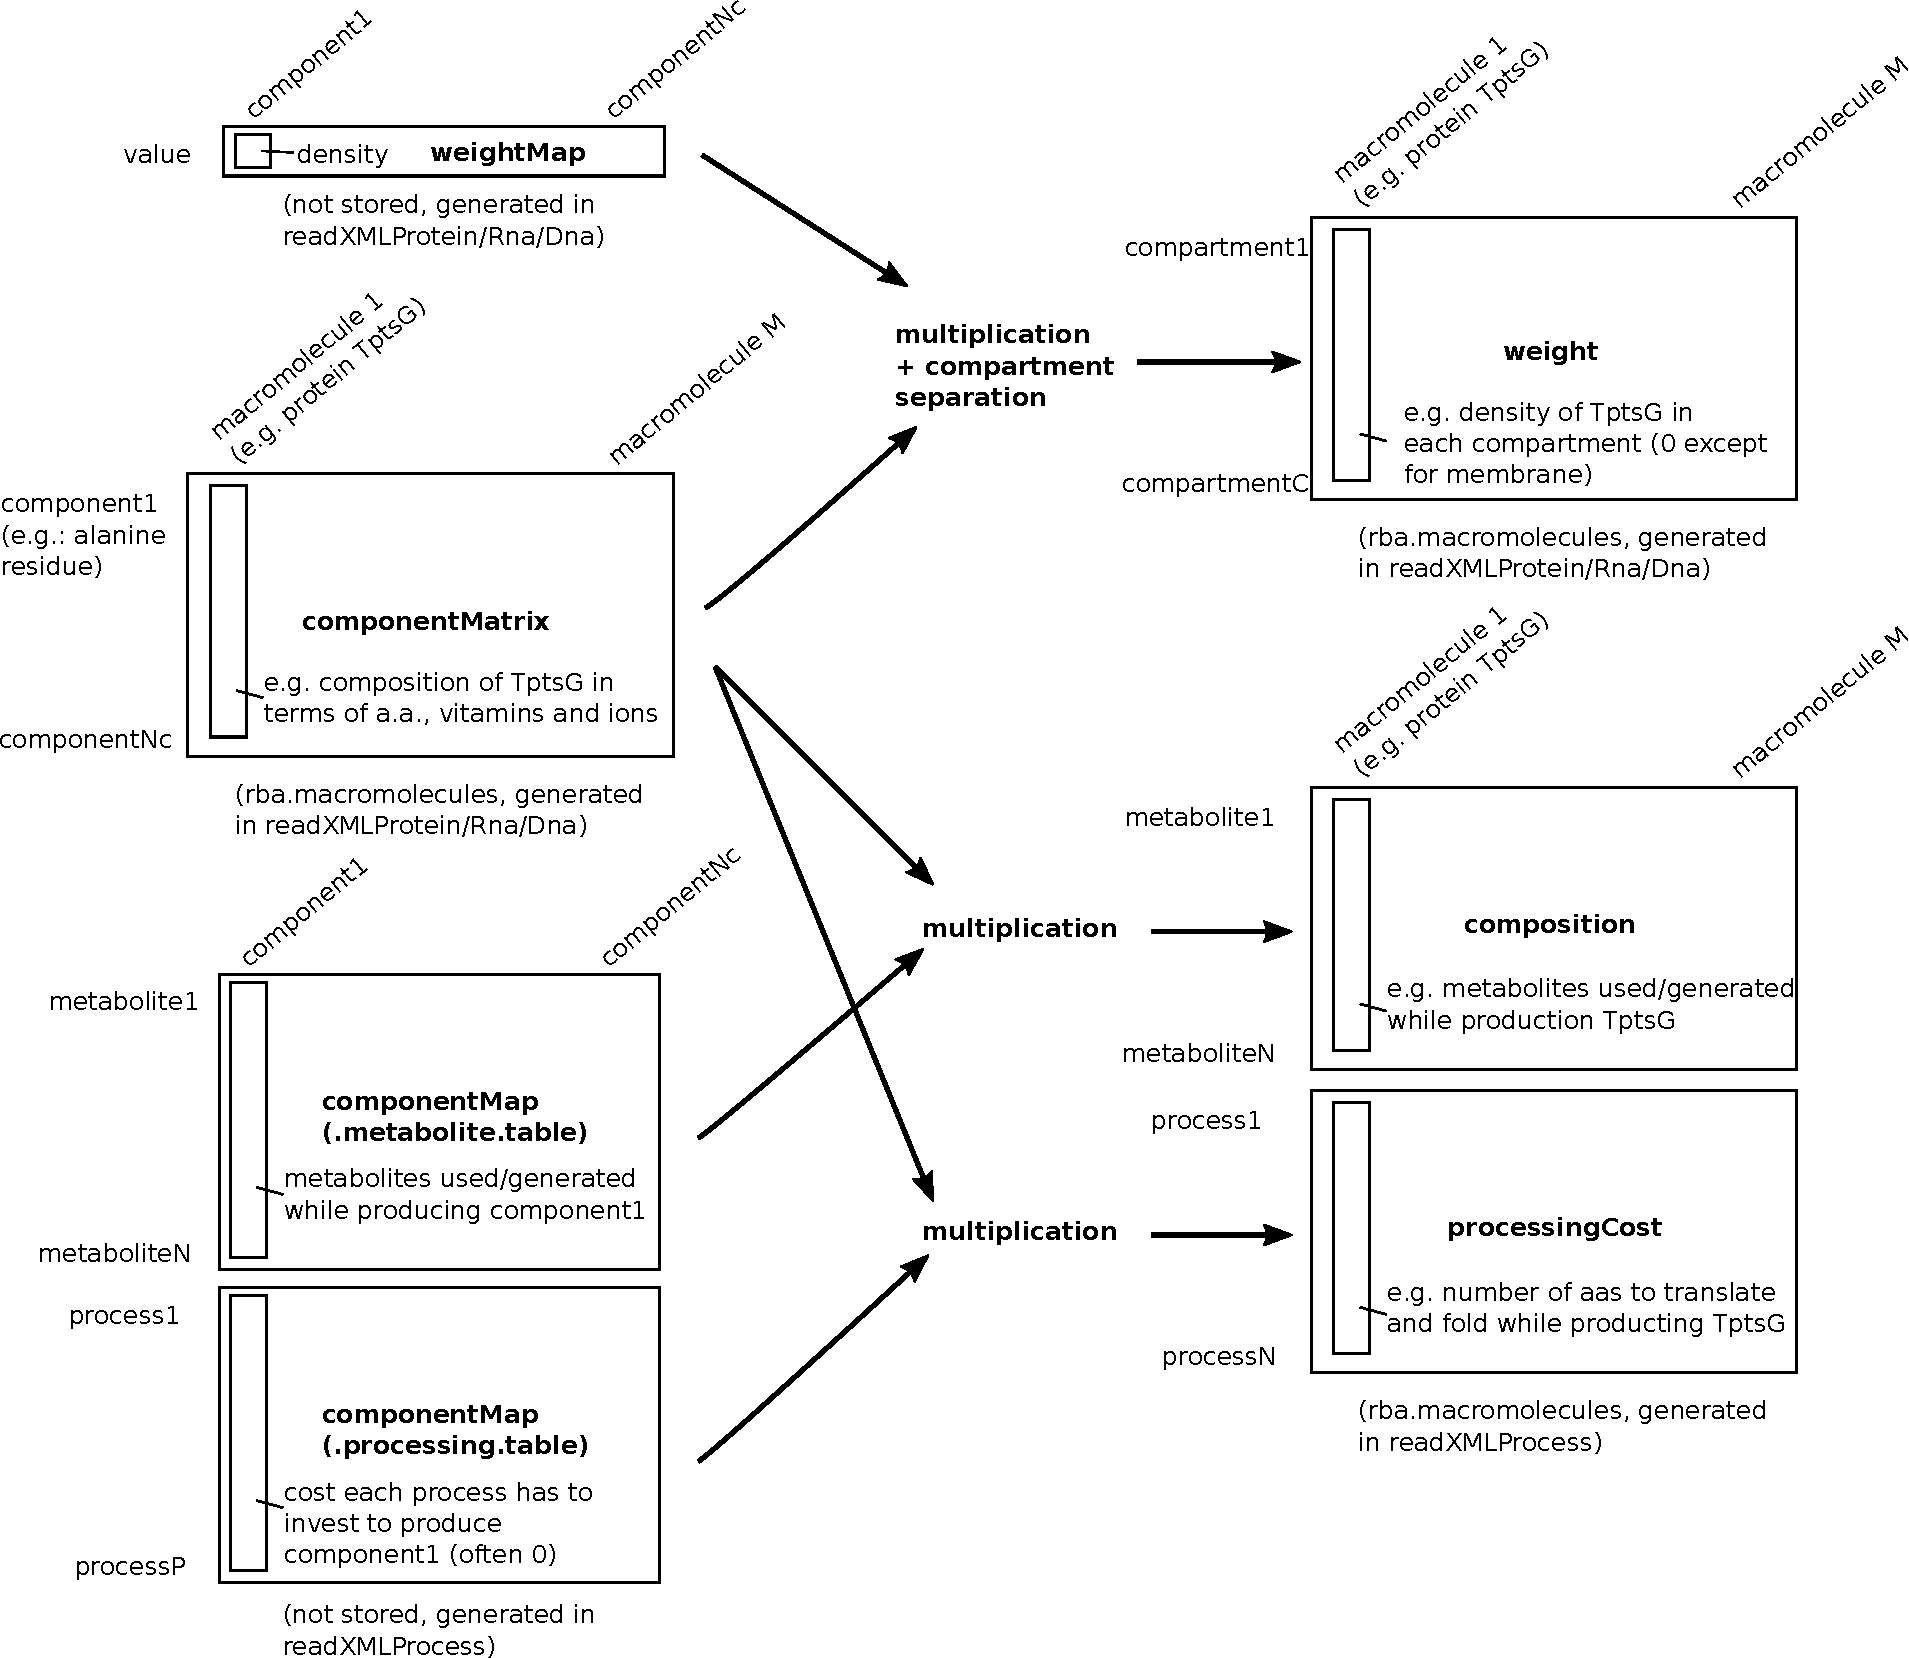
\includegraphics[width=\linewidth]{composition_matrices}
  \caption{Macromolecule matrices.}
  \label{fig:composition_matrices}
\end{figure}


\paragraph{Process-related matrices} \reffigt{fig:process_matrices} shows how the matrices stored in \texttt{rba.processes} are built.
\begin{figure}[ht]
  \centering
  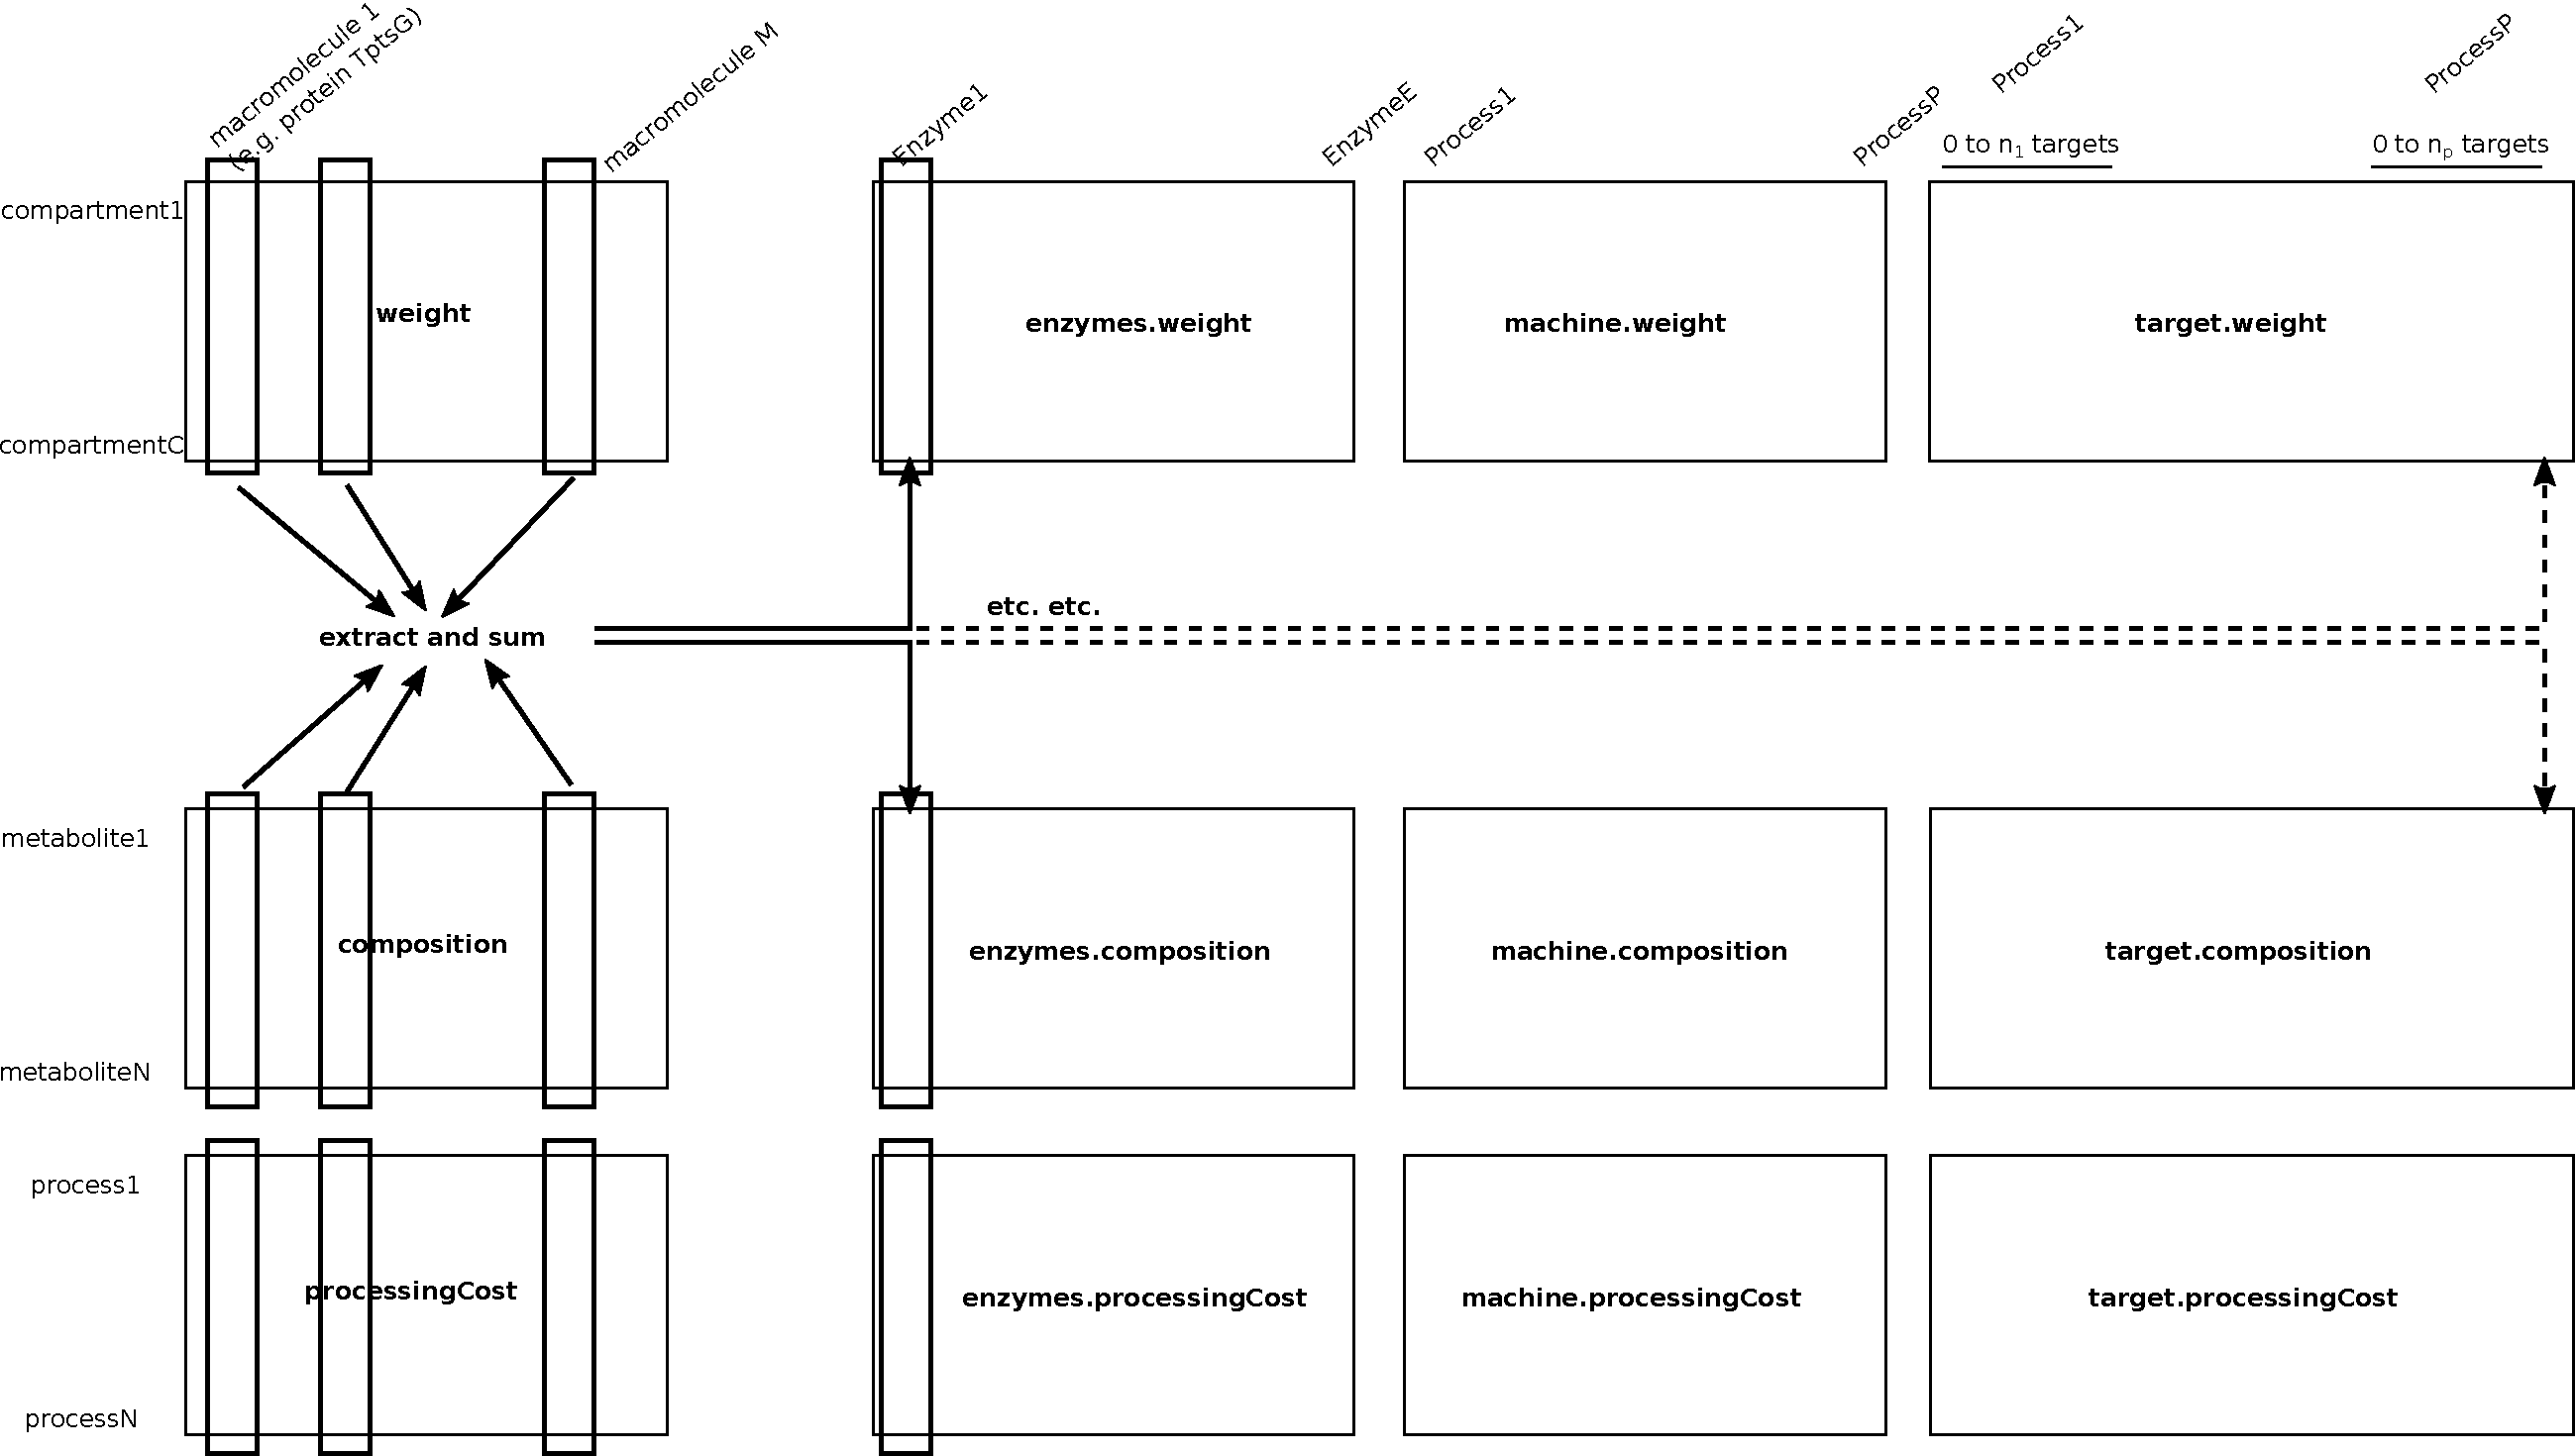
\includegraphics[width=\linewidth]{process_matrices}
  \caption{Process-related matrices.}
  \label{fig:process_matrices}
\end{figure}

\subsection{Building final matrices} \reffigt{fig:optimization_matrices} shows how the optimization matrices stored are built.
\begin{figure}[ht]
  \centering
  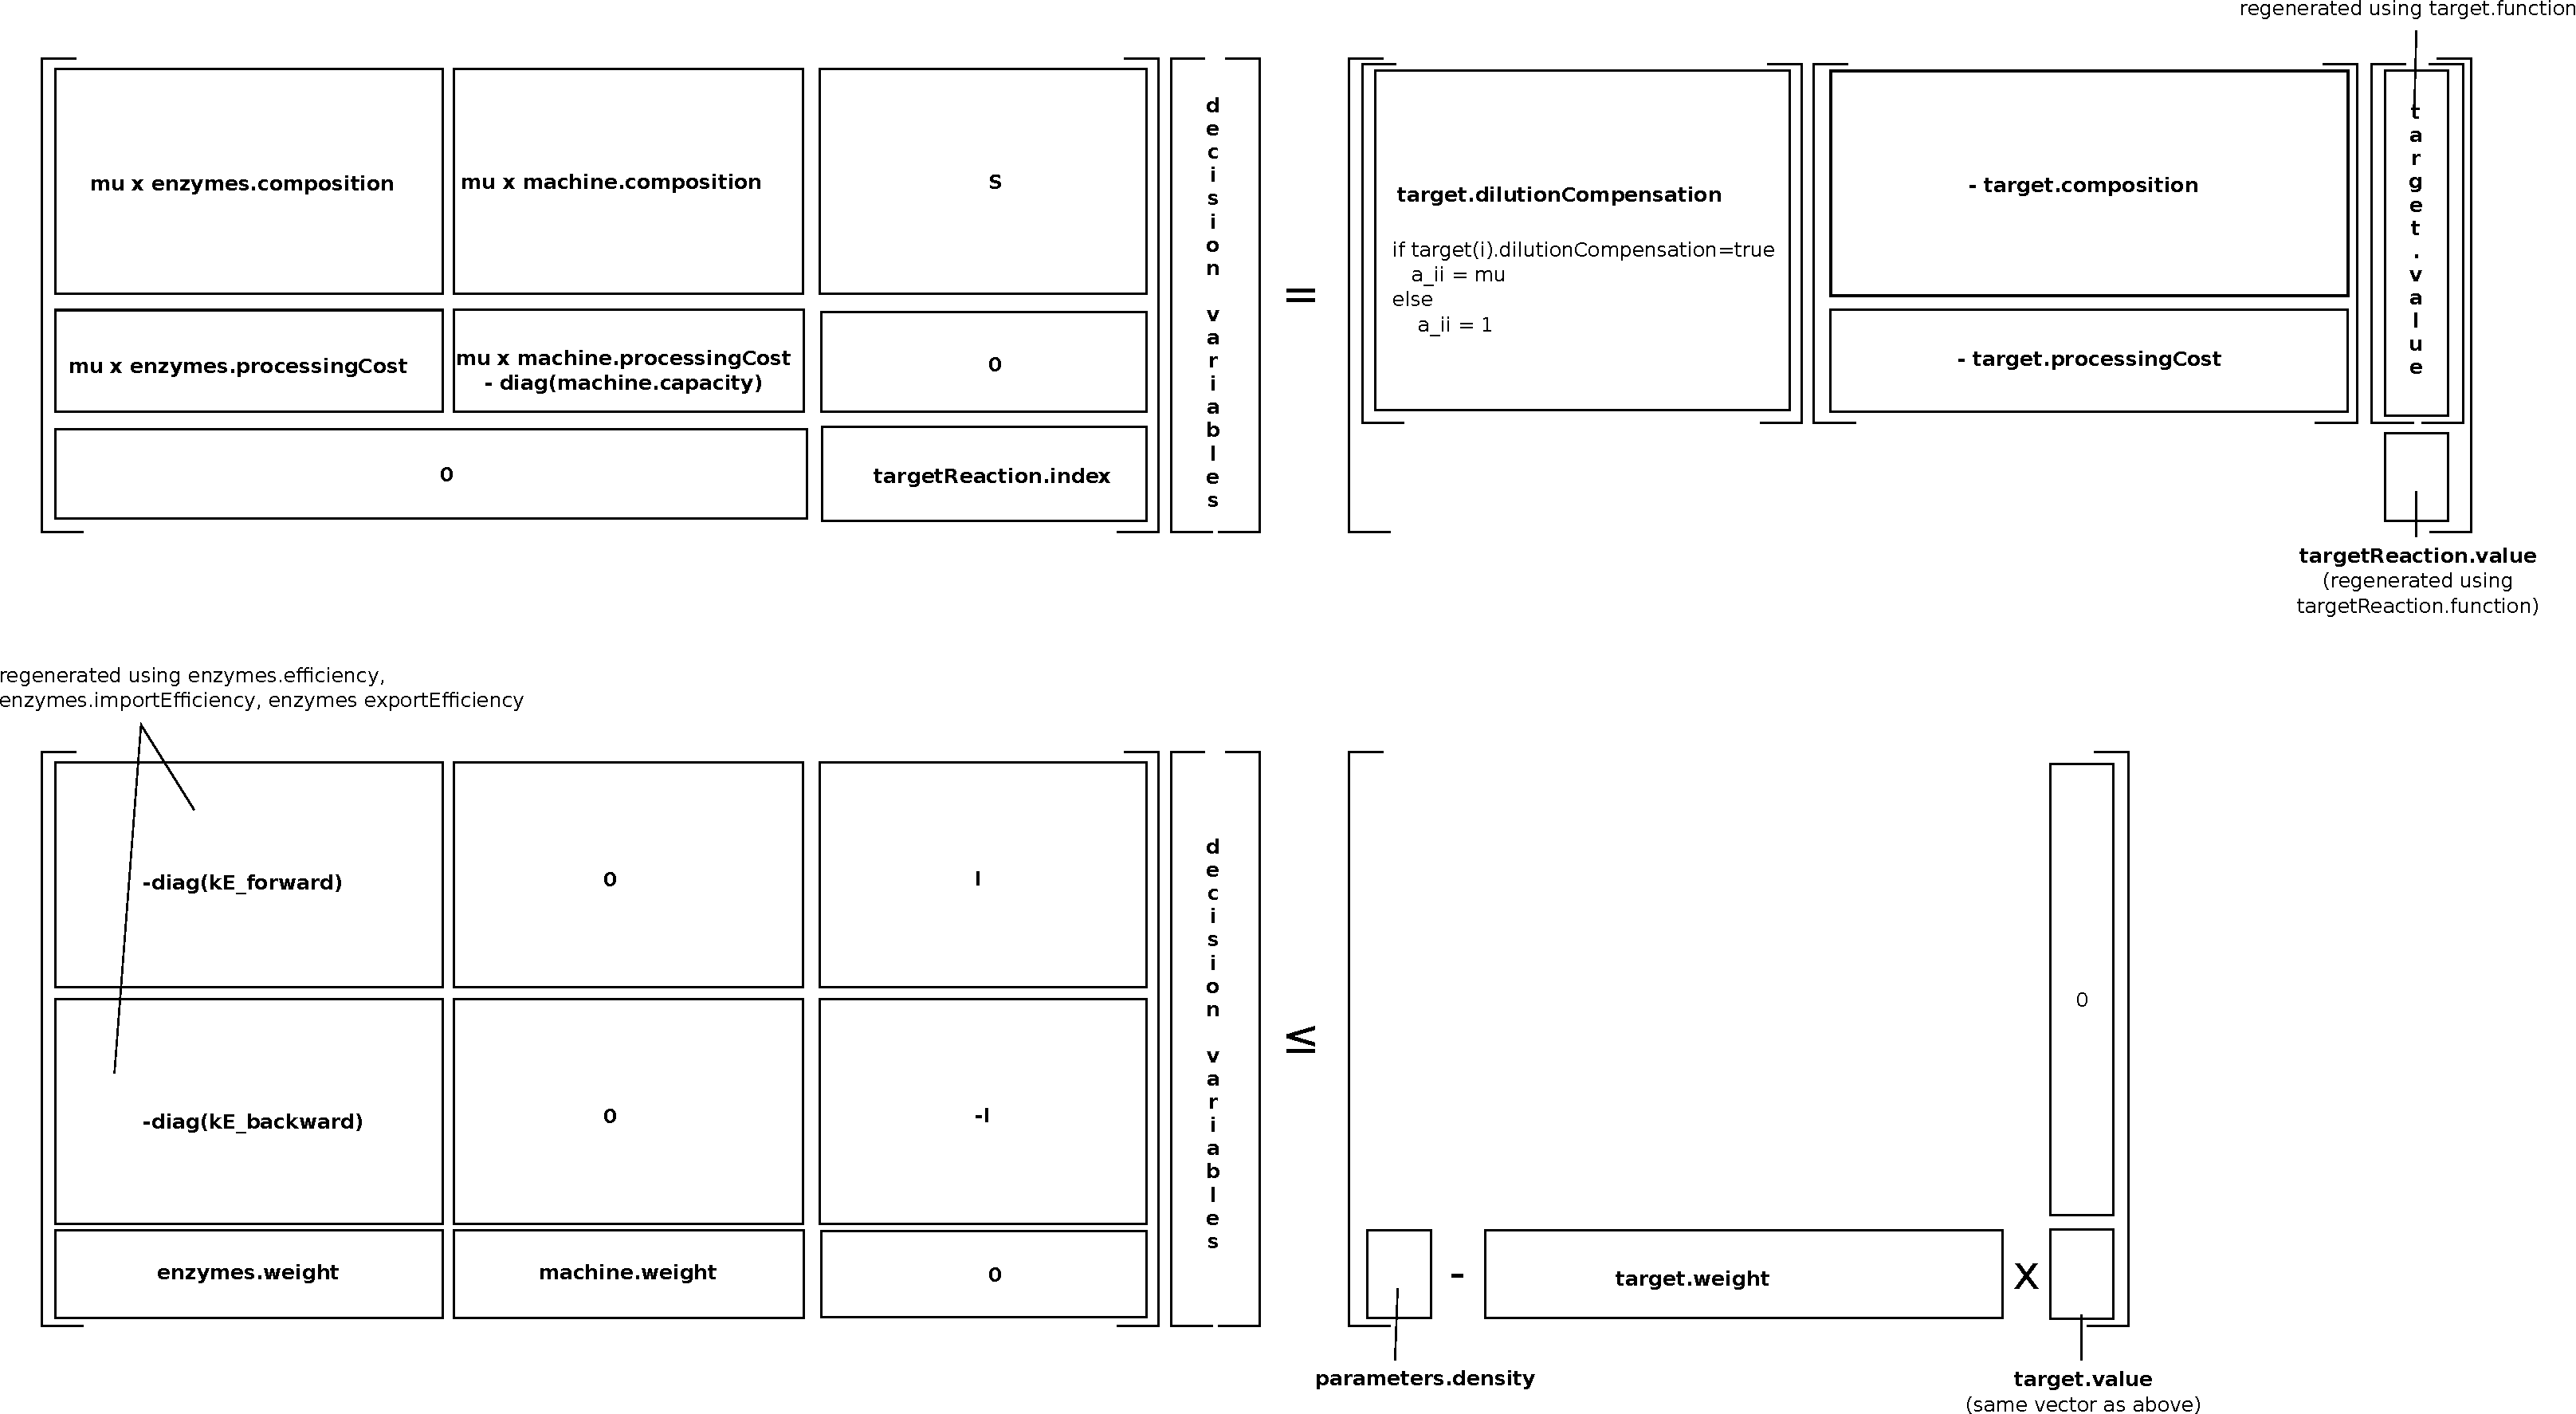
\includegraphics[width=\linewidth]{optimization_matrices}
  \caption{Matrices used to solve the optimization problem.}
  \label{fig:optimization_matrices}
\end{figure}
